\documentclass{beamer}
\usepackage{tbagrelbeamer}
\usepackage{beamerstyleceylan}

\newcommand{\tech}[1]{\tt{#1}}
\newcommand{\relief}[1]{{\color{structureTextColor} #1}}
\newcommand{\blue}[1]{{\color{regularblue} #1}}
\newcommand{\green}[1]{{\color{regulargreen} #1}}

\newcommand{\noeud}[1]{\blue{#1}}
\newcommand{\bit}[1]{{\small \green{#1}}}
\newcommand{\feuille}[2]{\tt{\large #2}~|~\tt{\blue{#1}}}

\usetikzlibrary{arrows.meta}


\theoremstyle{theoreme}
\newtheorem{theoreme}{Théorème.~}

\title{Les données sont D\tss{1}}
\subtitle{\'Etude de méthodes de compression sans pertes}
\author{Thomas \sc{Bagrel}}
\institute{Lycée Henri \sc{Poincaré}, Nancy}
\date{\sc{tipe} session 2018}

\begin{document}

% \begin{frame}
%   \frametitle{\secname{}}
%   \framesubtitle{\subsecname{}}

% \end{frame}

\begin{frame}
  \titlepage{}
\end{frame}

\begin{frame}
  \frametitle{Aperçu}

  \tableofcontents % [pausesections]
\end{frame}

\section{Régularités et gains}

\subsection{Théorie}

\begin{frame}
  \frametitle{\secname{}}
  \framesubtitle{\subsecname{}}

  \relief{Compression des données sans pertes}
  \begin{itemize}
    \item \pause exploiter les régularités des données
    \item \pause données aléatoires : pas de gain
  \end{itemize}

  \pause
  \begin{theoreme}[Entropie de \sc{Shannon}]
  \[
    H(S) = -\sum_{i = 1}^n p_i \log_2(p_i)
  \]
  {\footnotesize $H(S)$ : nb. de bits moyen par symbole de la source }
  \end{theoreme}
  \begin{itemize}
    \item \pause une fois les données compressées (dérivées) une fois, plus aucune régularité
  \end{itemize}
\end{frame}

\subsection{\tech{zip} recursif}

\begin{frame}
  \frametitle{\secname{}}
  \framesubtitle{\subsecname{}}

  \relief{Expérience :} compresser récursivement un fichier avec le même algorithme (\tech{zip})

  \pause

  \begin{center}
    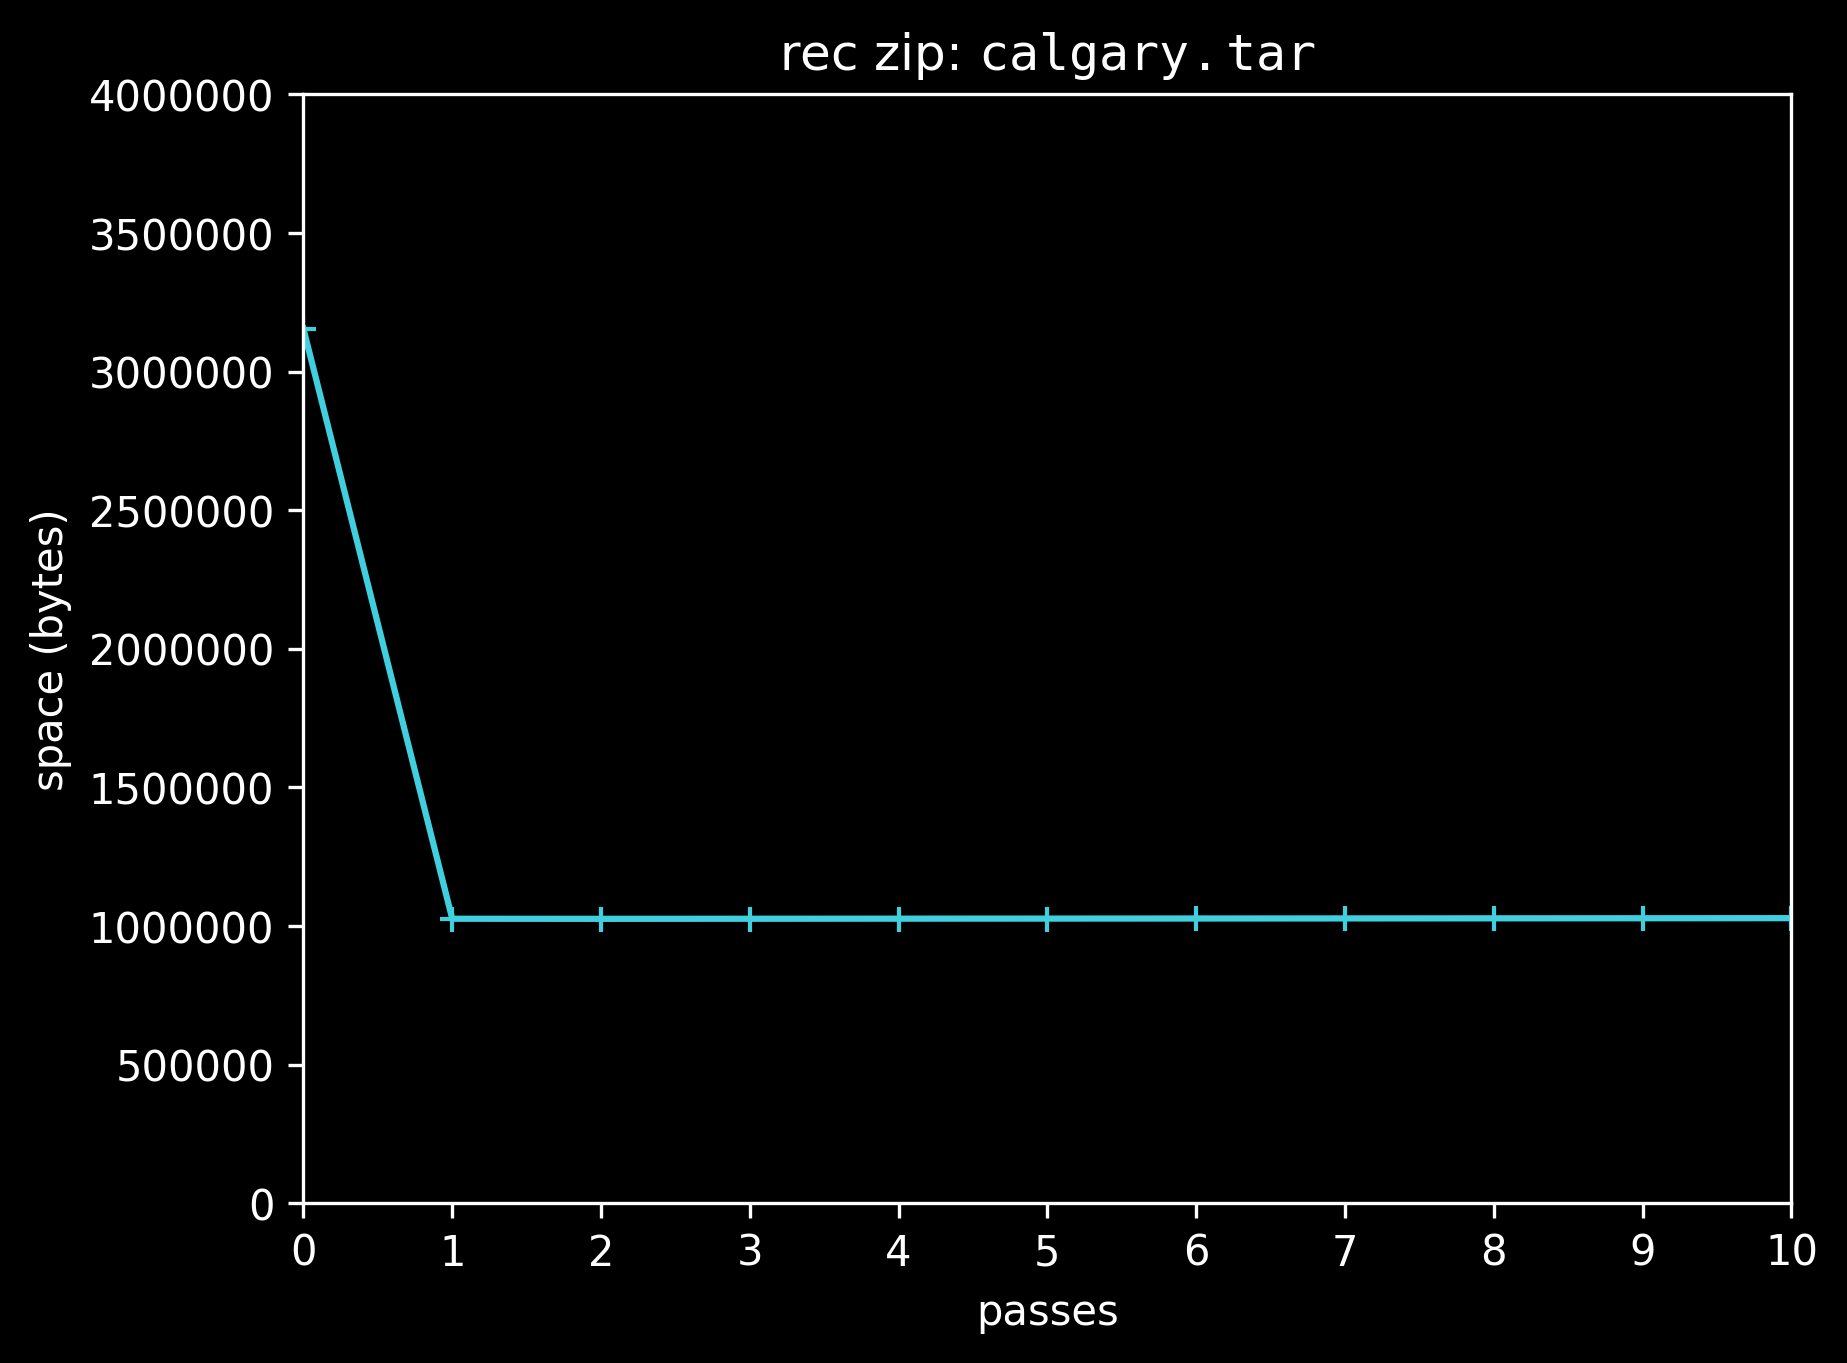
\includegraphics[scale=0.5]{rec_zip_measures.png}
  \end{center}
\end{frame}

\section{Composantes de la compression}

\begin{frame}
  \frametitle{\secname{}}

  \begin{center}
    \tikzset{%
      >={Latex[width=2mm,length=2mm]},
      % Specifications for style of nodes:
      base/.style = {%
        rectangle, rounded corners, draw=minigray, minimum width=6cm,
        minimum height=1.5cm, text centered, font=\sffamily\large},
      transform/.style = {%
        base},
    }
    \begin{tikzpicture}[node distance=2cm,
      every node/.style={fill=extragray, font=\sffamily}, align=center]
      \node (transform) [transform] {(~Transformée~)};
      \pause
      \draw[->] (transform) -- (model);
      \node (model) [base, below of=transform] {\blue{Modèle}};
      \pause
      \draw[->] (model) -- (coding);
      \node (coding) [base, below of=model] {\green{Codage}};
    \end{tikzpicture}
  \end{center}

\end{frame}

\section{Codage}
\subsection{Problème résolu}

\begin{frame}
  \frametitle{\secname{}}
  \framesubtitle{\subsecname{}}
  Le codage, contrairement aux apparences, est un problème \relief{résolu}
  \begin{itemize}
    \item\pause Si les $p_i$ sont connus, la limite de compression théorique est donnée par \sc{Shannon}
    \item\pause \sc{Huffman} permet d'\relief{approcher} cette limite
    \item\pause Le codage arithmétique l'\relief{atteint}
  \end{itemize}
\end{frame}

\begin{frame}
  \frametitle{\secname{}}
  \framesubtitle{\subsecname{}}
  Le codage arithmétique sera détaillé plus loin.

  \relief{Codage d'\sc{Huffman}} pour \tt{turlututu}
  \begin{center}
    \tikzset{%
      >={Latex[width=2mm,length=2mm]},
      % Specifications for style of nodes:
      base/.style = {%
        circle, draw=minigray, text centered,
        font=\sffamily},
    }
    \begin{tikzpicture}[scale=0.9, every node/.style={scale=0.9}]
      \node[draw] at (8, 0) (l_1) [base] {\feuille{1}{l}};
      \node[draw] at (10, 0) (r_1) [base] {\feuille{1}{r}};

      \node[draw] at (13, 1) (t_3) [base] {\feuille{3}{t}};
      \node[draw] at (3, 2) (u_4) [base] {\feuille{4}{u}};
      \pause

      \node[draw] at (9, 1) (empty_2) [base] {\noeud{2}};
      \draw (l_1) -- node[above left, midway] {\bit{0}} (empty_2);
      \draw (r_1) -- node[above right, midway] {\bit{1}} (empty_2);
      \pause

      \node[draw] at (11, 2) (empty_5) [base] {\noeud{5}};
      \draw (empty_2) -- node[above left, midway] {\bit{0}} (empty_5);
      \draw (t_3) -- node[above right, midway] {\bit{1}} (empty_5);
      \pause

      \node[draw] at (7, 3) (empty_9) [base] {\noeud{9}};
      \draw (u_4) -- node[above left, midway] {\bit{0}} (empty_9);
      \draw (empty_5) -- node[above right, midway] {\bit{1}} (empty_9);
      \pause

      \node at (2, 0.75) [above right] {\small\relief{Codes}};
      \node at (2, 0.30) [above right] {\small \tt{l}};
      \node at (5, 0.30) [above left] {\bit{100}};
      \node at (2, -0.05) [above right] {\small \tt{r}};
      \node at (5, -0.05) [above left] {\bit{101}};
      \node at (2, -0.40) [above right] {\small \tt{t}};
      \node at (5, -0.40) [above left] {\bit{11}};
      \node at (2, -0.75) [above right] {\small \tt{u}};
      \node at (5, -0.75) [above left] {\bit{0}};
    \end{tikzpicture}
  \end{center}
\end{frame}

\subsection{Inefficacité de \sc{Huffman} -- pourquoi}

\begin{frame}
  \frametitle{\secname{}}
  \framesubtitle{\subsecname{}}
  En pratique, efficacité de \relief{30 \%}
  \pause

  \bigskip

  En appliquant directement \sc{Shannon} aux \relief{fréquences} d'apparition,
  on commet des erreurs
  \begin{itemize}
    \item\pause un symbole n'est pas \relief{indépendant} des précédents
    \item\pause par exemple, en Français, q$\to$\blue{u} est plus fréquent que q$\to$\blue{z}
    \item\pause en quelque sorte, on oublie le caractère \relief{lipschitzien} de nos données
  \end{itemize}
  \pause

  \relief{Il faut donc un modèle}

\end{frame}

\section{Modèles généraux}
\subsection{\tech{bitwise encoder} et \tech{\sf{ppm}}}
\subsection{\tech{bitwise ppm} et \tech{bitwise ppm flat}}

\section{Impact de la transformée}
\subsection{\tech{\sc{bwt}} régularise nos données}
\subsection{En action avec la \tech{\sc{rle}}}

\section{Résultats finaux}

\end{document}